\documentclass[oneside, 10pt, notitlepage]{book}
	
	
\usepackage{../_mypackages/monographpreamble}
\usepackage{../_mypackages/commands}

\title{Special Relativity} % \MyTitle
\author{Bruno Murino} % \MyAuthor
\date{\today} % \MyDate

\usepackage{../_mypackages/monographstyle}

\graphicspath{ {figures/} }

%--------------------------------------------------------------------------------------------------

\begin{document}
\chapter{Lista IX}

\section*{Ex. 5)}

If
\eq{A\exp{iax}+B\exp{ibx}=C\exp{icx}}
then
\eq{A+B = C \qq{and} a=b=c}
where \(A\), \(B\), \(C\), \(a\), \(b\) and \(c\) are non-zero constants.\par 

\begin{proof}
    Let \(x=0\), then \(A+B=C\).\par 
    Plug in this result, giving
    \eq{A\exp{iax} + B\exp{ibx} = A\exp{icx} + B\exp{icx}}
    then
    \eq{A\lr{\exp{iax}-\exp{icx}} = -B\lr{\exp{ibx}-\exp{icx}}}
    Take the derivative once and let \(x=0\)
    \eq{A\lr{a-c} = -B\lr{b-c}}
    Take the derivative again and let \(x=0\)
    \eq{A\lr{a^2 - c^2} = -B\lr{b^2 - c^2} }
    \eq{A\lr{a-c}\lr{a+c} = -B\lr{b-c}\lr{b+c}}
    \eq{A\lr{a-c}\lr{a+c} = A\lr{a-c}\lr{b+c}}
    \eq{A\lr{a-c}\ssb{(a+c)-(b+c)}=0}
    \eq{A\lr{a-c}\lr{a-b}=0}
    So either \(a=c\) or \(a=b\). Assume \(a=c\), then the first derivative on \(x=0\) yields \(A(a-c) = 0 = -B(b-c)\), meaning \(b=c=a\). On the other hand, assume \(a=b\), then the first derivative on \(x=0\) yields 
    \eq{A(a-c) = -B(b-c) = -B(a-c)}
    \eq{(A+B)(a-c)=0}
    then either \(A=-B\) or \(a=c\). But if \(A=-B\) then \(C=0\) since \(A+B=C\), but we already know that \(C\) is a non-zero constant, thus the only option left is \(a=c\).\par 
    
    Thus \(a=b=c\) is the only solution.\par 
\end{proof}

\section*{Ex. 6)}

The Maxwell's equations on a conductor are
\begin{subequations}
    \begin{align}[left = \empheqlbrace\,]
    & \div{\vb{E}} = \frac{\rho_f}{\epsilon} \\
	& \div{\vb{B}} = 0 \\
	& \curl{\vb{E}} = -\pdv{\vb{B}}{t} \\
	& \curl{\vb{B}} = \mu \epsilon \pdv{\vb{E}}{t} + \mu \vb{J}_f
    \end{align}
\end{subequations}
Since the material is an ohmic conductor, we also have Ohm's law
\eq[eq:ohmlaw]{\vb{J}_f = \sigma \vb{E}}
Finally, we always have the charge conservation law
\eq[eq:chargecons]{\div{\vb{J}_f} + \pdv{\rho_f}{t}=0}\par 

Plugging \eqref{eq:ohmlaw} on \eqref{eq:chargecons} we find
\eq{\div{\lr{\sigma \vb{E}}} = -\pdv{\rho_f}{t}}
Plugging Gauss' law
\eq{\sigma \frac{\rho_f}{\epsilon} = -\pdv{\rho_f}{t}}
which we can solve to find
\eq{\rho_f(t) = \rho_f(0) \lexp{-\frac{\sigma}{\epsilon}t}}
This result implies that any charge concentration will rapidly vanish. We can assume this transient solution vanishes vary fast, so that we can assume \(\rho_f=0\), letting our Maxwell's equations as follows:
\begin{subequations}
    \begin{align}[left = \empheqlbrace\,]
    & \div{\vb{E}} =0 \\
	& \div{\vb{B}} = 0 \\
	& \curl{\vb{E}} = -\pdv{\vb{B}}{t} \\
	& \curl{\vb{B}} = \mu \epsilon \pdv{\vb{E}}{t} + \mu \vb{J}_f
    \end{align}
\end{subequations}\par 

Lets plug Ohm's law on Ampère's law:
\eq{\curl{\vb{B}} = \mu \epsilon \pdv{\vb{E}}{t} + \mu \sigma \vb{E}}
then take the derivative with respect to time:
\eq{\curl{\lr{\pdv{\vb{B}}{t}}} = \mu \epsilon \pdv[2]{\vb{E}}{t}+\mu \sigma \pdv{\vb{E}}{t}}
Plugging Faraday's law
\eq{-\curl{\lr{\curl{\vb{E}}}} = \mu \epsilon \pdv[2]{\vb{E}}{t}+\mu \sigma \pdv{\vb{E}}{t}}
Using the identity
\eq{\curl{\lr{\curl{\vb{E}}}} = \grad{\lr{\div{\vb{E}}}} - \laplacian{\vb{E}}}
we find
\eq{-\grad{\lr{\div{\vb{E}}}} + \laplacian{\vb{E}}=\mu \epsilon \pdv[2]{\vb{E}}{t}+\mu \sigma \pdv{\vb{E}}{t}}
But since we made \(\rho_f = 0\), it's simply
\eq{\laplacian{\vb{E}}=\mu \epsilon \pdv[2]{\vb{E}}{t}+\mu \sigma \pdv{\vb{E}}{t}}
and this is the wave equation for the electric field on a conductor.\par 

Let \(\vb{E}\) be a plane wave such that
\eq{\vb{E}=\vb{E}_0 \exp{i\lr{\vb{k}\cdot \vb{x}-\omega t}}}
then
\eq{\laplacian{\vb{E}} = -k^2 \vb{E}}
\eq{\pdv[2]{\vb{E}}{t}=-\omega^2 \vb{E}}
\eq{\pdv{\vb{E}}{t} = -i\omega \vb{E}}
Plugging this plane wave on the wave equation we find the dispersion relation
\eq{k^2 = \mu \epsilon \omega^2 - i\omega \sigma \mu}\par 

\section*{Ex. 7)}

Lets derive whats the Poynting vector on a material with dielectric constant \(\epsilon\) and magnetic susceptibility \(\mu\) from Ampère-Maxwell's law
\eq[a]{\curl{\vb{H}} = \vb{J}+\pdv{\vb{D}}{t}}
and from energy conservation
\eq[b]{\div{\vb{S}} + \pdv{u}{t} + \vb{E}\cdot \vb{J}=0}\par 

First, lets remember that 
\eq{u = \frac{1}{2}\lr{\vb{H}\cdot\vb{B}+\vb{D}\cdot\vb{E}}}
and lets take its derivative with respect to time
\eq{\pdv{u}{t} = \hlf \lr{\pdv{\vb{H}}{t}\cdot\vb{B} + \vb{H}\cdot\pdv{\vb{B}}{t} + \pdv{\vb{D}}{t}\cdot\vb{E} + \vb{D}\cdot\pdv{\vb{E}}{t} }}
Lets assume the material is linear, meaning
\eq{\vb{D}=\epsilon \vb{E} \qq{and} \vb{H} = \frac{1}{\mu}\vb{B}}
Plugging this on the derivative of EM energy, we find
\eq{\pdv{u}{t} = \frac{1}{\mu}\pdv{\vb{B}}{t}\cdot \vb{B} + \epsilon \pdv{\vb{E}}{t}\cdot \vb{E}}
Now we can merge the constants such that
\eq{\pdv{u}{t} = \vb{H}\cdot\pdv{\vb{B}}{t}+ \vb{E}\cdot\pdv{\vb{D}}{t}}

Lets multiply \eqref{a} by \(\vb{E}\):
\eq{\vb{E}\cdot \curl{\vb{H}} = \vb{E}\cdot\vb{J}+\vb{E}\cdot\pdv{\vb{D}}{t}}
then use the identity
\eq{\div{\lr{\vb{E}\cross \vb{H}}} = \vb{H}\cdot \curl{\vb{E}} - \vb{E}\cdot \curl{\vb{H}}} 
along with Faraday's law
\eq{\curl{\vb{E}}=-\pdv{\vb{B}}{t}}
to find
\eq{-\vb{H} \cdot \pdv{\vb{B}}{t} - \div{\lr{\vb{E}\cross\vb{H}}} = \vb{E}\cdot\vb{J}+\vb{E}\cdot \pdv{\vb{D}}{t}}
Rearranging we find
\eq{\div{\lr{\vb{E}\cross\vb{H}}} + \lr{\vb{H} \cdot \pdv{\vb{B}}{t} +\vb{E}\cdot \pdv{\vb{D}}{t} } + \vb{E}\cdot\vb{J} = 0}
We can recognise the middle term as \(\pdv*{u}{t}\), then
\eq{\div{\lr{\vb{E}\cross\vb{H}}} + \pdv{u}{t} + \vb{E}\cdot\vb{J} = 0}
which is exactly \eqref{b} if
\eq{\vb{S}=\vb{E}\cross\vb{H}}\par 

\section*{Ex. 8)}

The refraction index is defined as
\begin{equation}
    n = \frac{c}{v} = \frac{\sqrt{\mu \epsilon}}{\sqrt{\mu_ 0 \epsilon_0}}
\end{equation}
The situation is described on figure \ref{fig:obliqueincidence}.
\begin{figure}[H]
    \centering
    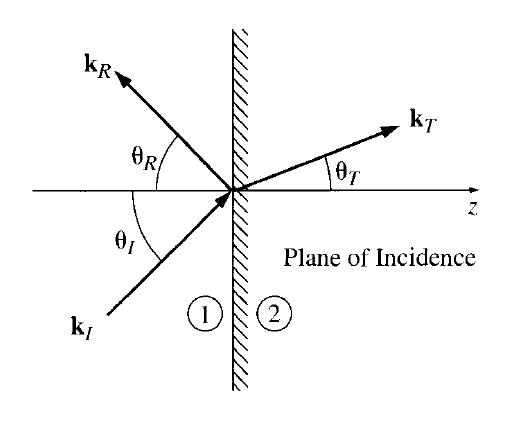
\includegraphics[width=0.4\textwidth]{griffithselectro9-14}
    \caption{Oblique incidence}
    \label{fig:obliqueincidence}
\end{figure}
where \(I\), \(R\) and \(T\) refer to the incident, reflected and transmitted wave, respectively. It is important to note that all three waves have the same frequency \(\omega\).
There are three fundamental laws of geometrical optics, and they are
\begin{enumerate}
    \item The incident, reflected and transmitted wave vectors form a plane (called the plane of incidence), which also includes the normal to the surface and the angle of incidence, the angle of reflection and the angle of transmission (of refraction) are all measured with respect to the normal.
    \item Law of reflection, which says that the angle of incidence is equal to the angle of reflection
    \(\theta_I = \theta_R\)
    \item Snell's law 
    \(n_1 sin\theta_I = n_2 sin\theta_T\)
\end{enumerate}
You'll have the three waves, and each of them can be decomposed into a perpendicular to the surface component and into a parallel to the surface component. The Fresnel's equations relate the amplitude of each of these components.

The boundary condition at the surface of change of media can be derived from Maxwell's laws on the absence of free sources
\begin{subequations}
    \begin{align}[left = \empheqlbrace\,]
    & \div{\vb{D}} = 0 \\
	& \div{\vb{B}} = 0 \\
	& \curl{\vb{E}} = -\pdv{\vb{B}}{t} \\
	& \curl{\vb{H}} = \pdv{\vb{D}}{t}
    \end{align}
\end{subequations}
and are
\begin{equation} D_{I_{\perp}} + D_{R_{\perp}}= D_{T_{\perp}}\end{equation}
\begin{equation} E_{I_{\parallel}} + E_{R_{\parallel}} = E_{T_{\parallel}}\end{equation}
\begin{equation} B_{I_{\perp}} + B_{R_{\perp}} = B_{T_{\perp}}\end{equation}
\begin{equation} H_{I_{\parallel}} + H_{R_{\parallel}} = H_{T_{\parallel}}\end{equation}
where \(D_{I_{\perp}}\) is the perpendicular component of the incident \(D\) field, for example.

The boundary conditions result in the Fresnel's equations
\begin{equation} 
    \frac{E_{R_{\parallel}}}{E_{I_{\parallel}}} = \frac{(n_1/\mu_1)cos\theta_T - (n_2/\mu_2)cos\theta_I}{(n_1/\mu_1)cos\theta_T + (n_2/\mu_2)cos\theta_I}
\end{equation}
\begin{equation} 
    \frac{E_{R_{\perp}}}{E_{I_{\perp}}} = \frac{(n_1/\mu_1)cos\theta_I - (n_2/\mu_2)cos\theta_T}{(n_1/\mu_1)cos\theta_I + (n_2/\mu_2)cos\theta_T}
\end{equation}
\begin{equation} 
    \frac{E_{T_{\parallel}}}{E_{I_{\parallel}}}  = \frac{2(n_1/\mu_1)cos\theta_I}{(n_1/\mu_1)cos\theta_T + (n_2/\mu_2)cos\theta_I}
\end{equation}
\begin{equation} 
    \frac{E_{T_{\perp}}}{E_{I_{\perp}}} = \frac{2(n_1/\mu_1)cos\theta_I}{(n_2/\mu_2)cos\theta_I + (n_1/\mu_1)cos\theta_T}
\end{equation}
where \(E_{R_{\parallel}}\) is the parallel component of the electric field of the reflected wave, for example. We this, you can construct the resulting waves. For example, the total amplitude of the reflected wave is \(E_R^2 = E_{R_{\parallel}}^2 + E_{R_{\perp}}^2\).

If \(\mu_1 = \mu_2 = \mu\), using Snell's law we can write
\begin{equation} 
    \frac{E_{R_{\parallel}}}{E_{I_{\parallel}}} = -\frac{tan(\theta_I - \theta_T)}{tan(\theta_I + \theta_T)}
\end{equation}
\begin{equation} 
    \frac{E_{R_{\perp}}}{E_{I_{\perp}}} = -\frac{sin(\theta_I - \theta_T)}{sin(\theta_I + \theta_T)}
\end{equation}
\begin{equation} 
    \frac{E_{T_{\parallel}}}{E_{I_{\parallel}}} = \frac{2sin\theta_I\theta_T}{sin(\theta_I + \theta_T)cos(\theta_I - \theta_T)}
\end{equation}
\begin{equation} 
    \frac{E_{T_{\perp}}}{E_{I_{\perp}}} = \frac{2sin\theta_I\theta_T}{sin(\theta_I + \theta_T)}
\end{equation}

Relating the intensity of the waves, we have that
\begin{equation} 
    I_I = \frac{1}{2}\epsilon_1 v_1 E_I^2 cos\theta_I
\end{equation}
\begin{equation} 
    I_R = \frac{1}{2}\epsilon_1 v_1 E_R^2 cos\theta_I
\end{equation}
\begin{equation} 
    I_T = \frac{1}{2}\epsilon_2 v_2 E_T^2 cos\theta_T
\end{equation}
noting that the cosines appear because we are looking at the intensity that gets to the surface, so we don't look the intensity parallel to it, we look only at the perpendicular intensity.
We define the reflection coefficient as
\begin{equation}
    R = \frac{E_R}{E_I}
\end{equation}
We define the transmission coefficient as
\begin{equation}
    T = \frac{E_T}{E_I}
\end{equation}














% \backmatter
% \printbib
\end{document}
	